%++++++++++++++++++++++++++++++++++++++++
\documentclass[article, 12pt]{article}
\usepackage{float}
\usepackage{setspace}
\usepackage{tabu} % extra features for tabular environment
\usepackage{amsmath}  % improve math presentation
\usepackage{graphicx} % takes care of graphic including machinery
\usepackage[margin=1in]{geometry} % decreases margins
\usepackage{cite} % takes care of citations
\usepackage[final]{hyperref} % adds hyper links inside the generated pdf file
\usepackage{tikz}
\usepackage{caption} 
\usepackage{fancyhdr}
\usepackage{amssymb} % symbols like /therefore
\usepackage{amsthm} % proofs
\usepackage{enumerate} % lettered lists
\usepackage{mathtools} % macros
\usepackage{tkz-graph}
\usepackage[colour, all, curve, arc, frame]{xy} % for diagrams
\usetikzlibrary{scopes}
% \usepackage{xcolor} \pagecolor[rgb]{0.12549019607,0.1294117647,0.13725490196} \color[rgb]{0.82352941176,0.76862745098,0.62745098039} % dark theme
\theoremstyle{definition}
\newtheorem{example}{Example}[subsubsection]
\newtheorem*{remark}{Remark}
\newtheorem{theorem}{Theorem}[subsubsection]
\newtheorem{definition}{Definition}[subsubsection]
\newtheorem{corollary}{Corollary}[subsubsection]
\hypersetup{
	colorlinks=false,      % false: boxed links; true: colored links
	linkcolor=blue,        % color of internal links
	citecolor=blue,        % color of links to bibliography
	filecolor=magenta,     % color of file links
	urlcolor=blue         
}
\usepackage{physics}
\usepackage{siunitx}
\usepackage{tikz,pgfplots}
\usepackage[outline]{contour} % glow around text
\usetikzlibrary{calc}
\usetikzlibrary{angles,quotes} % for pic
\usetikzlibrary{arrows.meta}
\usetikzlibrary{automata}
\tikzset{>=latex} % for LaTeX arrow head
\contourlength{1.2pt}

\colorlet{xcol}{blue!70!black}
\colorlet{vcol}{green!60!black}
\colorlet{myred}{red!70!black}
\colorlet{myblue}{blue!70!black}
\colorlet{mygreen}{green!70!black}
\colorlet{mydarkred}{myred!70!black}
\colorlet{mydarkblue}{myblue!60!black}
\colorlet{mydarkgreen}{mygreen!60!black}
\colorlet{acol}{red!50!blue!80!black!80}
\tikzstyle{CM}=[red!40!black,fill=red!80!black!80]
\tikzstyle{xline}=[xcol,thick,smooth]
\tikzstyle{mass}=[line width=0.6,red!30!black,fill=red!40!black!10,rounded corners=1,
                  top color=red!40!black!20,bottom color=red!40!black!10,shading angle=20]
\tikzstyle{faded mass}=[dashed,line width=0.1,red!30!black!40,fill=red!40!black!10,rounded corners=1,
                        top color=red!40!black!10,bottom color=red!40!black!10,shading angle=20]
\tikzstyle{rope}=[brown!70!black,very thick,line cap=round]
\def\rope#1{ \draw[black,line width=1.4] #1; \draw[rope,line width=1.1] #1; }
\tikzstyle{force}=[->,myred,very thick,line cap=round]
\tikzstyle{velocity}=[->,vcol,very thick,line cap=round]
\tikzstyle{Fproj}=[force,myred!40]
\tikzstyle{myarr}=[-{Latex[length=3,width=2]},thin]
\def\tick#1#2{\draw[thick] (#1)++(#2:0.12) --++ (#2-180:0.24)}
\DeclareMathOperator{\sn}{sn}
\DeclareMathOperator{\cn}{cn}
\DeclareMathOperator{\dn}{dn}
\def\N{80} % number of samples in plots


\usepackage{titling}
\renewcommand\maketitlehooka{\null\mbox{}\vfill}
\renewcommand\maketitlehookd{\vfill\null}
\usepackage{siunitx} % units
\usepackage{verbatim} 
\newcommand{\courseNumber}{MATH 263}
\newcommand{\courseName}{Discrete Mathematics 2}
\newcommand{\professor}{Dr. Petrescu}
\newcommand{\psetName}{Homework 3}
\newcommand{\dueDate}{Due: March 3, 2023}
\newcommand{\name}{Denny Cao}
\pagestyle{fancy}
\fancyhf{}% clears all header and footer fields
\fancyfoot[C]{--~\thepage~--}
\renewcommand*{\headrulewidth}{0.4pt}
\renewcommand*{\footrulewidth}{0pt}
\lhead{\name}
\chead{\courseNumber: \courseName}
\rhead{\professor}
\newcounter{questionNumber}

% Theorems for problem and answer
\newtheorem{question}{Question}
\newtheorem{answer}{Answer}

\fancypagestyle{plain}{%
  \fancyhf{}% clears all header and footer fields
  \fancyfoot[C]{--~\thepage~--}%
  \renewcommand*{\headrulewidth}{0pt}%
  \renewcommand*{\footrulewidth}{0pt}%
}

% Shortcuts
\DeclarePairedDelimiter\ceil{\lceil}{\rceil} % ceil function
\DeclarePairedDelimiter\floor{\lfloor}{\rfloor} % floor function

\DeclarePairedDelimiter\paren{(}{)} % parenthesis

\newcommand{\df}{\displaystyle\frac} % displaystyle fraction
\newcommand{\qeq}{\overset{?}{=}} % questionable equality

\newcommand{\Mod}[1]{\;\mathrm{mod}\; #1} % modulo operator

\newcommand{\comp}{\circ} % composition

% Sets
\DeclarePairedDelimiter\set{\{}{\}}
\newcommand{\unite}{\cup}
\newcommand{\inter}{\cap}

\newcommand{\reals}{\mathbb{R}} % real numbers: textbook is Z^+ and 0
\newcommand{\ints}{\mathbb{Z}}
\newcommand{\nats}{\mathbb{N}}
\newcommand{\rats}{\mathbb{Q}}

\newcommand{\degree}{^\circ}

% Counting
\newcommand\perm[2][^n]{\prescript{#1\mkern-2.5mu}{}P_{#2}}
\newcommand\comb[2][^n]{\prescript{#1\mkern-0.5mu}{}C_{#2}}

% Relations
\newcommand{\rel}{\mathcal{R}} % relation

\setlength\parindent{0pt}

% Directed Graphs
\usetikzlibrary{arrows}
\tikzset{vertex/.style = {shape=circle,draw,minimum size=1.5em}}
\tikzset{edge/.style = {->,> = latex'}}

%++++++++++++++++++++++++++++++++++++++++
% title stuff

\makeatletter
\renewcommand{\maketitle}{\bgroup\setlength{\parindent}{0pt}
    \begin{flushleft}
        \textbf{\@title} \\ \vskip0.2cm
        \begingroup
            \fontsize{14pt}{12pt}\selectfont
            \courseNumber: \courseName 
            \vskip0.3cm 
            \professor
        \endgroup \vskip0.3cm
        \@date \hfill\rlap{}\bf{\name} \\ \vskip0.1cm
        \hrulefill
    \end{flushleft}\egroup 
}
\makeatother

\title{\Huge\bf{\psetName}}
\author{\name}
\date{\dueDate}

\author{\name}
\date{\dueDate}

\begin{document}
    \maketitle
    \thispagestyle{empty}

    % Question 1
    \begin{question}
        Solve the traveling salesperson problem for this graph by finding the total weight of all Hamilton circuits and determining a circuit with minimum total weight.  
        \begin{figure}[H]
            \centering
            \xygraph{ !{<0cm,0cm>;<2cm,0cm>:<0cm,2cm>::} !~-{@{-}@[|(3)]@[red]}!{(0,0) }*+[blue]{\bullet_{a}}="a" !{(1,1) }*+[blue]{\bullet_{b}}="b" !{(2,1) }*+[blue]{\bullet_{c}}="c" !{(1,-1)}*+[blue]{\bullet_{d}}="d"  "a"-"c"_(0.7){7}  "a"-"b"^(0.5){3} "a"-"d"_(0.3){4} "d" -"b" ^(0.4){9}  "b"-"c"^(0.4){6}  "c"-"d"^(0.6){4} }
        \end{figure}
    \end{question}

    % Question 2
    \begin{question}
        Try to daw the given  graph without any crossings.  If it is not possible explain why.
        \begin{figure}[H]
            \centering
            \xygraph{ !{<0cm,0cm>;<2cm,0cm>:<0cm,2cm>::}!~-{@{-}@[|(2.5)]@[blue]} !{(2,2) }*+{\bullet_{a}}="a" !{(1,1) }*+{\bullet_{b}}="b" !{(2,0) }*+{\bullet_{e}}="e" !{(3,1)}*+{\bullet_{c}}="c"!{(0,0)}*+{\bullet_{d}}="d" !{(4,0)}*+{\bullet_{f}}="f"  "a"-"b" "a"-"c"  "a"-"e" "b"-"d" "f"-"b" "d"- "c"   "d"-"e"  "f"-"e" "f"-"c"  }
        \end{figure}
    \end{question}

    % Question 3
    \begin{question}
        An edge coloring of a graph is an assignment of colors to edges so that edges incident with a common vertex are assigned different colors. The edge chromatic number of a graph is the smallest number of colors that can be used in an edge coloring of the graph. The edge chromatic number of a graph G is denoted by $\chi(G)$.  Find the edge chromatic numbers of: \vskip.3cm\hskip1cm a) $C_n$, where  $n \ge 3$.\hskip3.5cm b) $W_n$, where $n \ge 3$.
    \end{question}

    % Question 4
    \begin{question}
        Find the edge chromatic number of $K_n$ when n is a positive integer.
    \end{question}

    % Answer 4
    \begin{answer}
    
    \end{answer}

    % Question 5
    \begin{question}
        Show that if $G$ is a bipartite simple graph with $v$ vertices and $e$ edges, then $e \leq \frac{v^2}4$.
    \end{question}

    % Question 6
    \begin{question}
        Suppose that you have a three-gallon jug and a five-gallon jug. You may fill either jug with water, you may empty either jug, and you may transfer water from either jug into the other jug. Use a path in a directed graph to show that you can end up with a jug containing exactly one gallon. [Hint: Use an ordered pair (a, b) to indicate how much water is in each jug. Represent these ordered pairs by vertices. Add an edge for each allowable operation with the jugs.]
    \end{question}

    % Question 7
    \begin{question}
        Find the number of paths of length n between any two adjacent vertices in $K_{3,3}$ for the values of $n$ in $\{3, 4, 5, 6\}$
    \end{question}

    % Question 8
    \begin{question}
        Determine whether  ({\em i}) Dirac's theorem can be used to show  the graphs below have a Hamilton circuit, ({\em ii}) whether Ore's theorem can be used and finally ({\em iii}) if the graph has a Hamilton circuit.
        \begin{figure}[H]
            \centering
            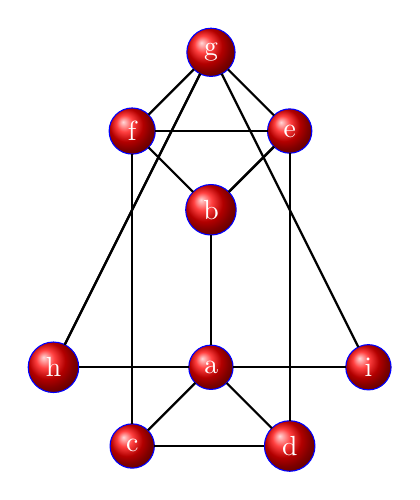
\begin{tikzpicture} \SetGraphUnit{1}\tikzset{VertexStyle/.style ={draw,shape = circle,shading= ball,ball color= red ,minimum size= 16pt,color= blue, text=white}};\coordinate (o) at (0,0);\SO(o){a} \NO(o){b} \SOEA(a){d}\SOWE(a){c}\NOEA(b){e} \NOWE(b){f}\NOEA(f){g}\NOWE(c){h}\NOEA(d){i}\Edges(a,b,f,e,d,a,b,e,g,h,g,i,a)\Edges(d,c,f)\Edges(b,e)\Edges(c,a,h)\Edges(g,f)\end{tikzpicture}
        \end{figure}
    \end{question}

    % Question 9
    \begin{question}
        Find the length of a shortest path between \{({\it x} and {\it z}),( {\it v} and {\it w}), ({\it t} and {\it z})\} in the weighted graph below, using Djikstra algorithm. Show each step.
        \begin{figure}[H]
            \centering
            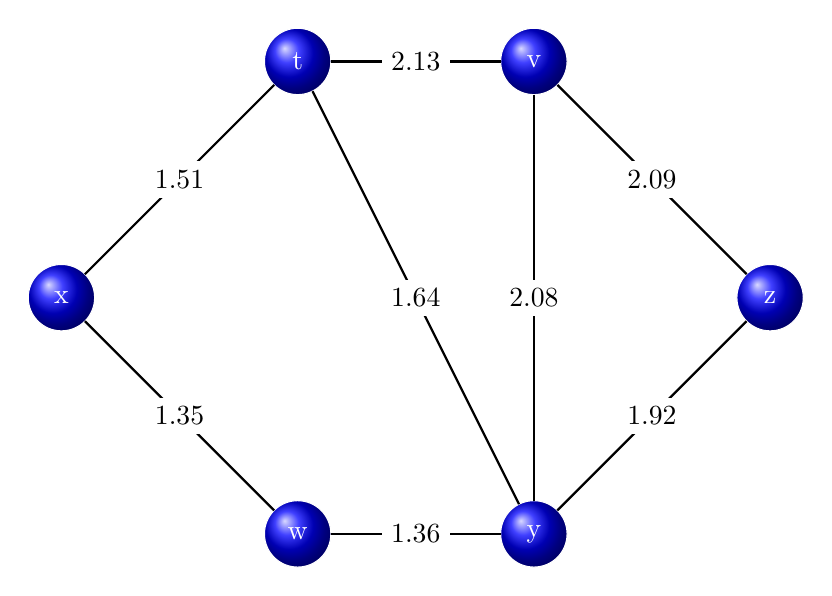
\begin{tikzpicture}\SetGraphUnit{3}\tikzset{VertexStyle/.style ={draw,shape = circle,shading= ball, ball color= blue,minimum size= 24pt, color= white}} \Vertex{x}\NOEA(x){t}\EA(t){v}\SOEA(v){z}\SOWE(z){y}\WE(y){w}\NOWE(w){x}\tikzset{LabelStyle/.style ={fill=white}}\Edge[label=$1.51$](x)(t)\Edge[label=$2.13$](t)(v)\Edge[label=$2.09$](v)(z)\Edge[label=$1.92$](y)(z)\Edge[label=$1.36$](w)(y)\Edge[label=$2.08$](v)(y)\Edge[label=$1.35$](x)(w)\Edge[label=$1.64$](t)(y)\end{tikzpicture}
        \end{figure}
    \end{question}
    
    % Question 10
    \begin{question}
        Prove the following statement: If H is a subgraph of G and G is a planar simple graph, then H is also planar.
    \end{question}

    % Quesion 11
    \begin{question}
        Find the  chromatic number, $\chi(G)$, of the graph below  and decide whether or not the graph is planar. Justify your answer.  
    
        \begin{figure}[H]
        \centering
            \xygraph{ !{<0cm,0cm>;<0cm,2cm>:<-2cm,0cm>::} !{(0,0);a(0)**{}?(1.0)}*{\bullet}="a1" !{(0,0);a(72)**{}?(1.0)}*{\bullet}="a2" !{(0,0);a(144)**{}?(1.0)}*{\bullet}="a3" !{(0,0);a(216)**{}?(1.0)}*{\bullet}="a4" !{(0,0);a(288)**{}?(1.0)}*{\bullet}="a5" !{(0,0);a(0)**{}?(1.8)}*{\bullet}="b1" !{(0,0);a(72)**{}?(1.8)}*{\bullet}="b2" !{(0,0);a(144)**{}?(1.8)}*{\bullet}="b3" !{(0,0);a(216)**{}?(1.8)}*{\bullet}="b4" !{(0,0);a(288)**{}?(1.8)}*{\bullet}="b5" "a1"-"a3" "a3"-"a5" "a5"-"a2" "a2"-"a4" "a4"-"a1" "b1"-"b2" "b2"-"b3" "b3"-"b4" "b4"-"b5" "b5"-"b1" "a1"-"b1" "a2"-"b2" "a3"-"b3" "a4"-"b4" "a5"-"b5" }
        \end{figure} 

    \end{question}
    % Question 12
    \begin{question}
        Prove that  Dijkstra's Algorithm  finds the length of the  shortest path between 2 vertices  of a  connected simple undirected  weighted  graph.\\ {\bf NOTE:} Check  the textbook.
    \end{question}
\end{document} 
